\documentclass[letterpaper,10pt,conference]{ieeeconf}
\IEEEoverridecommandlockouts
\overrideIEEEmargins
\usepackage{amsmath,amssymb,bm,graphicx,booktabs,array,url}
\usepackage[hidelinks]{hyperref}
\newcommand{\R}{\mathbb R}
\newcommand{\ind}{\mathbf 1}

\graphicspath{{../evidence/chapter3_interface_model/}{../evidence/chapter3_interface_online/}}
\title{Predicting Handoff Compatibility for Driving and Gap Crossing of a Single-Track Robot}
\author{\normalsize Research draft: author information pending}
\setlength{\textfloatsep}{10pt plus 2pt minus 2pt}
\setlength{\dbltextfloatsep}{10pt plus 2pt minus 2pt}
\begin{document}
\raggedbottom
\maketitle
\thispagestyle{plain}\pagestyle{plain}
\begin{abstract}
Crossing a gap does not complete a single-track traversal task if the landing state prevents the ground controller from continuing within the road corridor. We study this handoff through two learned interfaces while keeping the driving and jumping controllers frozen. An action-conditioned model predicts whether a valid handoff occurs and the distribution of the state delivered to the ground controller. A conditional outcome model evaluates whether that controller can complete the remaining task from the predicted state. The planner integrates these predictions over finite route, approach-speed, and preference candidates, with a separate outcome branch for ground-only routes. Supervised fitting uses 1,919 published executions partitioned by starting condition. On 540 development executions, the composed model achieves a completion Brier score of 0.1152 and conditional handoff-position RMSE of 0.132~m. In a subsequent Isaac simulation panel of 30 new starting conditions and three crossed-slot repetitions, however, it completes 15/90 tasks, compared with 33/90 for a direct classifier and 41/90 for a distance rule. All 33 selected detours time out. The results establish a working state-prediction and skill-composition interface, but also show that accurate average prediction does not ensure useful candidate rankings. A task-conditioned extension jointly selects approach and downstream road, then revises the road at measured handoff. In a separate 30-condition panel it completes 30/90 tasks, versus 28/90 without revision and 28/90 with fixed commands. Forty-four handoff decisions change, with eleven resulting completions. The intervals include no difference and incoming states differ across many pairs, so these outcomes demonstrate executable feedback rather than superior planning.
\end{abstract}
\noindent\textbf{Index terms:} Model learning for control; motion planning; skill composition; single-track robots.

\section{Introduction}
A single-track robot must maintain dynamic balance while steering toward a goal. A gap introduces a controller transition: ground driving prepares a jump, and the jumping skill returns a moving vehicle to ground control. Reaching the opposite bank is therefore an intermediate event. The state at contact must also allow the next controller to continue within the available road space.

This problem differs from evaluating each skill at its own nominal initial state. Approach commands alter the state entering the jump, and the jump changes the state from which driving resumes. A frozen controller can be competent in isolation yet receive unsuitable states when composed with another skill. Sequential behavior composition provides a foundation for reasoning about such interfaces~\cite{burridge1999}; here we examine a learned, finite-candidate approximation for a single-track platform.

The research question is whether predicting the distribution of handoff states and their downstream consequences can guide approach decisions. Our method separates the upstream distribution from a conditional full-task outcome predictor. It retains failed approaches as negative handoff examples and does not equate contact, controller switching, or short survival with goal completion. The term world model denotes this restricted predictor of action-conditioned physical outcomes; no visual generation or new low-level reinforcement learning is involved.

The implemented contribution is a two-interface prediction and planning system with explicit state outputs, grouped supervised training, and execution while the vehicle remains in motion. We evaluate prediction separately from online decisions and preserve a direct-success comparator and a distance rule. The evidence supports physical handoff prediction, task-dependent continuation, and executed feedback, while exposing candidate-ranking failures. It does not establish superior planning, a certified recoverability boundary, or generalization to new maps or corridor widths.

\section{Related Work}
\textbf{Composing locomotion behaviors.} Sequential behavior composition organizes dynamical controllers into larger tasks~\cite{burridge1999}. For wheeled bipeds, Xin and Vijayakumar combine rolling and contact-changing template models with online planning and whole-body control~\cite{xin2020}. Lee \emph{et al.} integrate learned locomotion and navigation for wheeled-legged robots~\cite{lee2024}. Our setting differs in morphology and interface: a single-track vehicle uses an existing ground controller and fixed jumping policy, while the upper layer evaluates their predicted event-level consequences. These precedents motivate composition, rather than establishing a claim to first introducing it.

\textbf{Learned models for planning.} PETS combines probabilistic dynamics with sampled uncertainty propagation~\cite{chua2018}. Yang \emph{et al.} study learned locomotion models and account for planning latency~\cite{yang2020}. DayDreamer learns world models for physical robots, including locomotion and navigation~\cite{wu2022}. Here, learning is supervised on simulator executions, and the action is a route--skill decision rather than a low-level control sequence. The model predicts the handoff state and conditional continuation outcome; it does not train an imagined policy. A direct success predictor is retained as a comparator: intermediate predictions should be evaluated beyond their ability to assign a final score.

\section{Task and System Interface}
\subsection{Common-goal traversal}
Let $\mathcal H$ be a known height map with support mask, $\mathcal R$ a finite road set, and $\mathcal G$ a shared goal. A task action is
\begin{equation}
 a=(r,v^\star,\alpha,\kappa),\quad r\in\mathcal R,\quad\kappa\in\{0,1\},
\end{equation}
where $v^\star$ and $\alpha$ specify approach speed and ground-controller preference, and $\kappa$ selects ground-only traversal or a ground--jump--ground sequence. Every route targets the same region. The robot continues moving during planning; stopping or restoring a saved physical state is not used to resolve a late decision.

The map contains a 0.30-m open gap, 1--4-mm surface stones outside the jump region, and 0.02-m and 0.08-m ridges. The four candidate routes share a destination while providing different approaches or a continuous-ground detour.

Task success requires reaching $\mathcal G$ at the declared minimum forward speed, without physical termination or any recorded corridor violation:
\begin{equation}
Y=\ind_{\mathcal G}\ind_{\mathrm{physical\ valid}}\ind_{\mathrm{corridor\ valid}}.
\label{eq:success}
\end{equation}
Far-bank contact is intermediate, not success. Bypasses need not generate flight or landing events. Failure endpoints and milestones are retained, so surviving briefly after contact is not conflated with task completion.

\subsection{Frozen controllers and handoff}
Ground motion uses the existing STTW H75 controller with ECBC/ESO and zero lower learned residual. Jumping uses a frozen heading-conditioned checkpoint, \texttt{heading125}. H75 adjusts speed/steering references from causal history and path preview above the balance controller and extended-state observer (ESO). Increasing $\alpha$ shifts the trained preference from path following toward speed tracking, with finite secondary costs and unchanged actuator limits. These identities are held fixed in the main study. At the jump-entry line, control switches to the jump policy; this line is distinct from observed takeoff. After far-bank contact, ground control resumes at the next 20-ms boundary. No physical state reset is performed. Controller initialization follows the existing handoff interface rather than assuming interchangeable ground and airborne histories.

The chosen $(v^\star,\alpha)$ controls approach. Postlanding motion uses fixed 1.5~m/s and $\alpha=0.5$, not separately optimized settings. The planning objective thus concerns the consequences of approach decisions for later continuation. The continuation predictor targets the final goal in~\eqref{eq:success}; it is not a dedicated estimator of stabilization distance.


\section{Handoff-Conditioned World Model}
\subsection{Inputs and event semantics}
Let $V_h$ denote a handoff that occurs without an earlier road violation. A failed approach or a missing handoff is a negative event label, even when no terminal state can be assigned. For a published candidate $a$, the model input is
\begin{equation}
 \xi=[x_t,o_t,c_t,t,a_{\rm enc},H_t]\in\R^{582},
\end{equation}
where $x_t$ is the 13-dimensional root state, $o_t$ the 80-dimensional current observation, and $c_t$ the 352-dimensional recorded ground-controller history. The remaining inputs are physical time, an eight-dimensional candidate encoding, and a 128-dimensional known-map crop. Candidate encoding describes the route and its speed, preference, and jump flag; it is not a motor command.

The map crop contains an $8\times8$ height grid and corresponding support mask sampled from the terrain mesh. The model therefore has access to known geometry, rather than inferred visual terrain. Normalization uses TRAIN statistics only. Unlike the earlier event-chain prototype, this model does not propagate a PCA history vector through successive predicted events.

The conditional output is a 39-dimensional handoff descriptor
\begin{equation}
 z_h=[x_h,f_h,t_h],
\end{equation}
with root state $x_h\in\R^{13}$, latest measured observation frame $f_h\in\R^{25}$, and physical handoff time $t_h$. Recorded event roots were checked against the corresponding physical transition. The frame is available before switching; it is not a future trajectory observation. This descriptor is an approximation to the closed-loop state, not a serialization of all joints, estimator history, or hidden contact-solver state.

\subsection{Upstream distribution and downstream outcome}
Three independently initialized MLPs, each with 128 and 64 SiLU hidden units, predict a diagonal Gaussian and two Bernoulli outputs:
\begin{equation}
 F_\theta(\xi)=(\mu_h,\log\sigma_h^2,p_h,p_g).
\end{equation}
There are 80 scalar outputs: 39 means, 39 log variances, valid-handoff probability $p_h$, and ground-route completion probability $p_g$. The ground output shares the trunk; it is a separate output head, not an independently fitted model.

A second three-member ensemble, with 64 and 32 SiLU hidden units, estimates
\begin{equation}
 R_\phi(z_h)=P(Y=1\mid V_h,z_h,I,\pi_{\rm H75}),
\end{equation}
where $I$ is the fixed cold-start initialization rule. H75, its postlanding speed and preference, and the downstream straight-road context are fixed. Thus $R_\phi$ estimates continuation to the original goal within this context, not a general recovery domain over arbitrary corridor widths, curves, or controller versions. A separate two-second continuation pilot is retained as diagnostic evidence and is not substituted for this full-goal target.

\subsection{Masked supervised training}
Let $J$ mark jump candidates and $G$ ground-only candidates. For normalized handoff targets, the upstream objective is
\begin{equation}
\begin{split}
\mathcal L_U={}&\operatorname{BCE}_{J}(p_h,V_h)
 +\operatorname{BCE}_{G}(p_g,Y)\\
 &+\tfrac12\mathbb E_{V_h=1}\left[
 \frac1{39}\sum_{d=1}^{39}
 \left((z_d-\mu_d)^2e^{-\ell_d}+\ell_d\right)\right],
\end{split}
\end{equation}
where $\ell_d$ is log variance clipped to $[-4,3]$. Missing states are excluded only from the conditional Gaussian loss. They remain classification examples; unsuccessful but valid handoffs train the downstream model with negative goal labels.

The upstream and direct-success networks are fitted for 250 epochs per member using Adam, learning rate $10^{-3}$ and weight decay $10^{-4}$. The downstream networks use the same optimizer settings for 200 epochs. Upstream checkpoints minimize the grouped DEV objective above; downstream and direct checkpoints minimize DEV Brier score. These different selection objectives are declared rather than treated as interchangeable. All three members use the same data split, so they are optimization realizations, not independent experimental datasets.

\section{Candidate Evaluation and Execution}
For jump candidates, complete-task probability is estimated by
\begin{equation}
 \widehat Q(s,a)=\widehat P(V_h\mid s,a)
 \int R_\phi(z)\widehat p_\theta(z\mid V_h,s,a)\,dz.
\label{eq:composition}
\end{equation}
The implementation averages this estimate over the three upstream members and 32 samples per member. Common Gaussian draws are used across candidates within a query. Sampled quaternions are normalized, sampled handoff time is bounded below by query time, and the latest-frame validity flag is set to one. These operations enforce representation conventions; they do not ensure dynamically realizable samples. Ensemble spread is not used as a certified risk margin.

Ground-only candidates are scored with $p_g$. No additional contact probability is multiplied into Eq.~\eqref{eq:composition}: the full-goal target already requires the relevant preceding physical events. The decomposition defines an estimator, not automatic probability calibration.

The planner evaluates 60 candidates: four route types, five speeds, and three preferences. The routes are straight crossing, S-bend crossing, right-angle crossing, and ground detour. Available speeds are 1.5, 1.8, 2.0, 2.3, and 2.6~m/s, with $\alpha\in\{0,0.5,1\}$. Route geometry and geometric admission are shared across methods. The highest-scoring admitted candidate is selected. Actual computation time is rounded up to a control interval while existing control continues, followed by a publication-time admission recheck. No physical state is restored to the query state.

The original panel performs one moving query and a publication recheck. A task-conditioned extension introduces a downstream road $g$ and evaluates
\begin{equation}
 (a^*,g^*)=\arg\max_{a,g}\;p_h(s,a)\mathbb E_{z\mid V_h,s,a}[R_\phi(z,g,I)].
\label{eq:joint}
\end{equation}
A single road is selected after averaging particles and ensemble members; maximizing separately for each imagined state would grant unavailable foresight. The extension uses the 15 straight-crossing speed/preference candidates and three downstream geometries. It therefore isolates interface decisions, rather than replacing the broader route panel. At actual handoff, feedback optionally replaces $g^*$ with $\arg\max_g R_\phi(z_h^{\rm measured},g,I)$. The planned road remains active during query latency. Postlanding speed/preference and all controller weights remain fixed.

\section{Experimental Design}
\subsection{Data and grouped fitting}
The initial collection contains 720 executions, partitioned by eight TRAIN and four DEV starting conditions. A second collection requests 1,440 executions at multiple query positions, of which 1,199 are published and attributable to the selected candidates. The 241 unpublished requests remain in the original record but are not assigned counterfactual candidate outcomes. This second collection uses six TRAIN and two DEV roots. Across the combined 20 roots, no exact initial-state duplicate crosses the split.

The resulting upstream dataset contains 1,379 TRAIN executions with 205 goals and 540 DEV executions with 79 goals. Valid handoffs provide 463 TRAIN and 168 DEV examples for the downstream model. All observed candidate failures remain in the corresponding classification denominators. A further 240 executions from four previously inspected roots provide historical transfer analysis, not an untouched confirmation set.

An initial model trained only at the early query position had a historical multi-position handoff-position RMSE of 2.32~m. Including the previously partitioned distance-training data was a declared development change. Neither that earlier fit nor its failure is discarded.

\subsection{Online panel and comparators}
Before online execution, model weights and 30 newly sampled starting conditions were frozen. Ten conditions are assigned to each query position $x\in\{1.8,3.0,5.0\}$~m. Initial lateral offset, yaw, and roll vary within $\pm0.03$~m, $\pm0.035$~rad, and $\pm0.02$~rad, respectively; initial speed lies in $[1.9,2.1]$~m/s. Each condition is evaluated three times per method, crossing methods over environment slots. Thus each method has 90 episodes but only 30 independent starting conditions.

The direct-success comparator uses the same 582-dimensional query input, grouped data, hidden widths, and three-member fitting budget, with a scalar goal output. The distance rule selects fixed candidates derived from the earlier TRAIN data for each query position. A TRAIN-only route-type completion prior and a constant completion prior are additional offline baselines. Controllers, physical task limits, and the ten-second observation horizon are common.

The primary outcome is complete-task success. Road violations and computation time are reported separately. Paired gains and losses include all matched condition--slot pairs. Confidence intervals resample starting conditions, stratified by query position, with 5,000 bootstrap samples; the three repetitions are averaged within each condition. Recorded query root states are compared across methods. Equality of these records does not certify equality of hidden PhysX solver state.

\section{Results}
\subsection{Physical interface and prediction}
The earlier stage audit found both approach and continuation failures. In the 720-execution collection, 265 executions did not reach jump entry; among 217 handoffs, 153 subsequently failed. Of those handoffs, 26 had already violated the road constraint. In the 1,199 published distance executions, 383 did not reach entry and 379 of 493 handoffs subsequently failed, with 53 prior road violations. These counts motivate both interfaces; they do not support assigning the entire bottleneck to landing recovery.

\begin{table}[t]
\centering\small
\caption{Completion Brier scores. DEV participates in checkpoint selection; historical transfer is previously inspected.}
\begin{tabular}{lrr}\toprule
Predictor & DEV (540)& Historical (240)\\\midrule
Two-interface & .11520 & .11139\\
Direct success & .12336 & .11839\\
Route-type prior & .11673 & .10998\\
Constant prior & .12490 & .12165\\\bottomrule
\end{tabular}
\label{tab:prediction}
\end{table}
The interface estimator has lower DEV Brier score than the direct comparator, but the route prior is competitive and has the lowest historical-transfer score (Table~\ref{tab:prediction}). Conditional handoff-position RMSE is 0.1317~m on DEV and 0.1299~m on historical transfer, computed over Cartesian components of valid handoffs. Handoff-time MAE is 0.3711 and 0.4588~s, respectively. These conditional errors exclude absent handoffs; they cannot replace occurrence evaluation or full-task outcomes.

\begin{figure*}[t]
\centering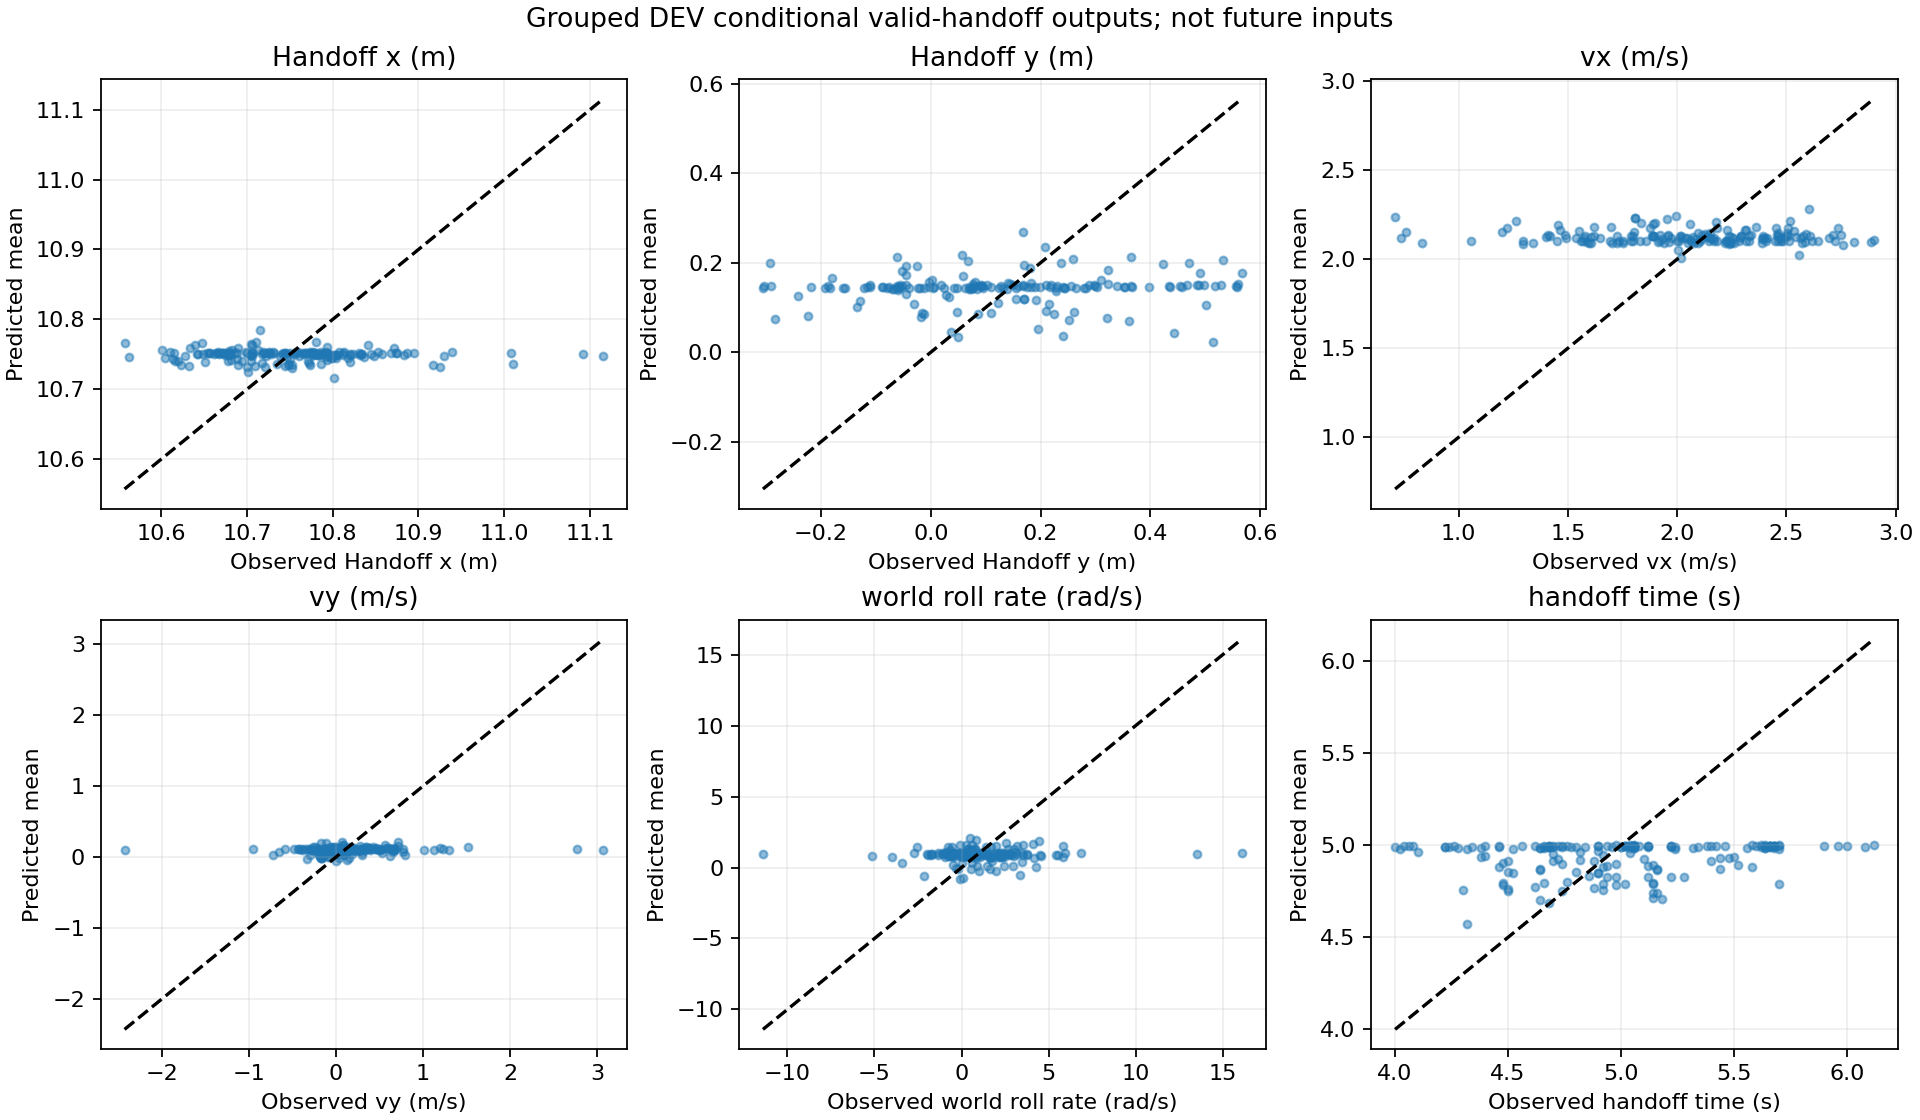
\includegraphics[width=.94\textwidth]{handoff_outputs.png}
\caption{Predicted and observed handoff outputs on 168 valid DEV handoffs. State regression is conditional on valid handoff; the event classifier also includes failed and missing handoffs. The plots expose physical prediction errors rather than only a final completion score.}
\label{fig:outputs}
\end{figure*}
\begin{figure}[t]
\centering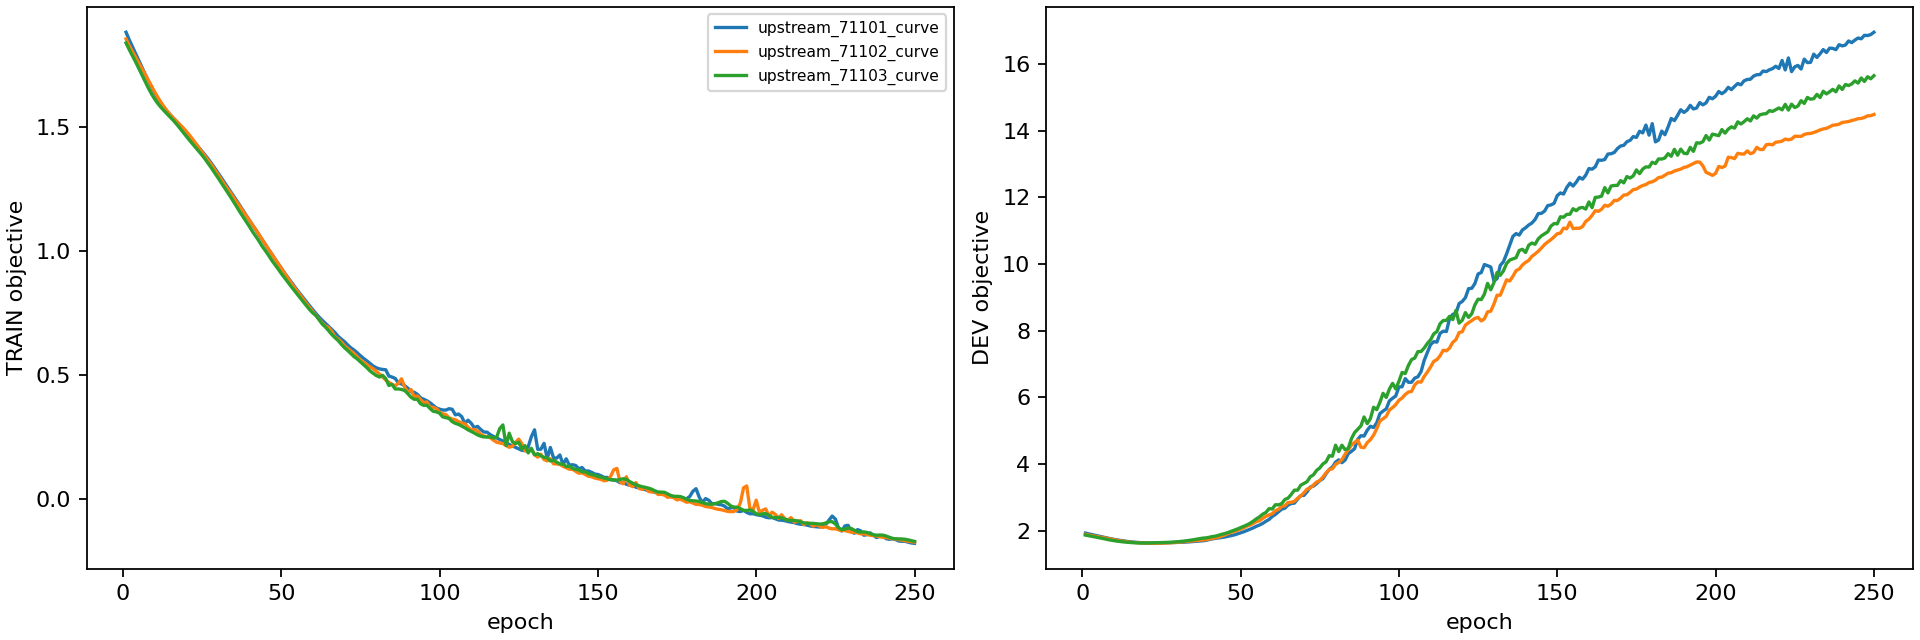
\includegraphics[width=.98\columnwidth]{training.png}
\caption{Recorded upstream/direct training and development curves. Upstream selection uses the masked joint objective; the direct comparator uses DEV Brier. Their numerical scales are not interchangeable.}
\end{figure}

\subsection{Information in the handoff state}
To test whether the continuation model uses more than elapsed time and nominal progress, we fitted three feature subsets on the same 463 TRAIN and 168 DEV valid handoffs. Each uses three 64--32 SiLU networks, 200 epochs, and the same grouped DEV checkpoint criterion. The geometric subset contains world $x,y$, mount-corrected yaw, forward velocity, and time. The dynamics extension adds roll, pitch, lateral and vertical velocity, and three world angular velocities. Existing root-only and latest-frame models are reused unchanged.
\begin{table}[t]
\centering\footnotesize
\caption{Conditional goal Brier by input subset. Historical sets were previously inspected; DEV selects epochs.}
\begin{tabular}{lrrr}\toprule
Inputs&DEV&Source&RB\\
&168&65&70\\\midrule
Time only&.21142&.18155&.18660\\
Geometry/speed/time&.19686&.14725&.15194\\
With dynamics&.14450&.13305&.13488\\
Root/time&.14178&.12881&.13602\\
Root/frame/time&.14502&.12531&.13610\\\bottomrule
\end{tabular}
\label{tab:information}
\end{table}
Adding dynamics lowers Brier relative to geometry/speed/time in all six DEV roots and both historical sets (Table~\ref{tab:information}). Time alone performs near the constant prior. Thus measured handoff dynamics contains predictive information in the fixed downstream context. This is a grouped feature diagnostic, not an isolated causal effect of lean: several state fields and input parameter counts change together. The latest observation frame does not consistently improve on the physical root alone. Predictive information at observed handoffs does not establish that sampling those states upstream improves candidate selection.

\subsection{Executed decisions}
\begin{figure*}[t]
\centering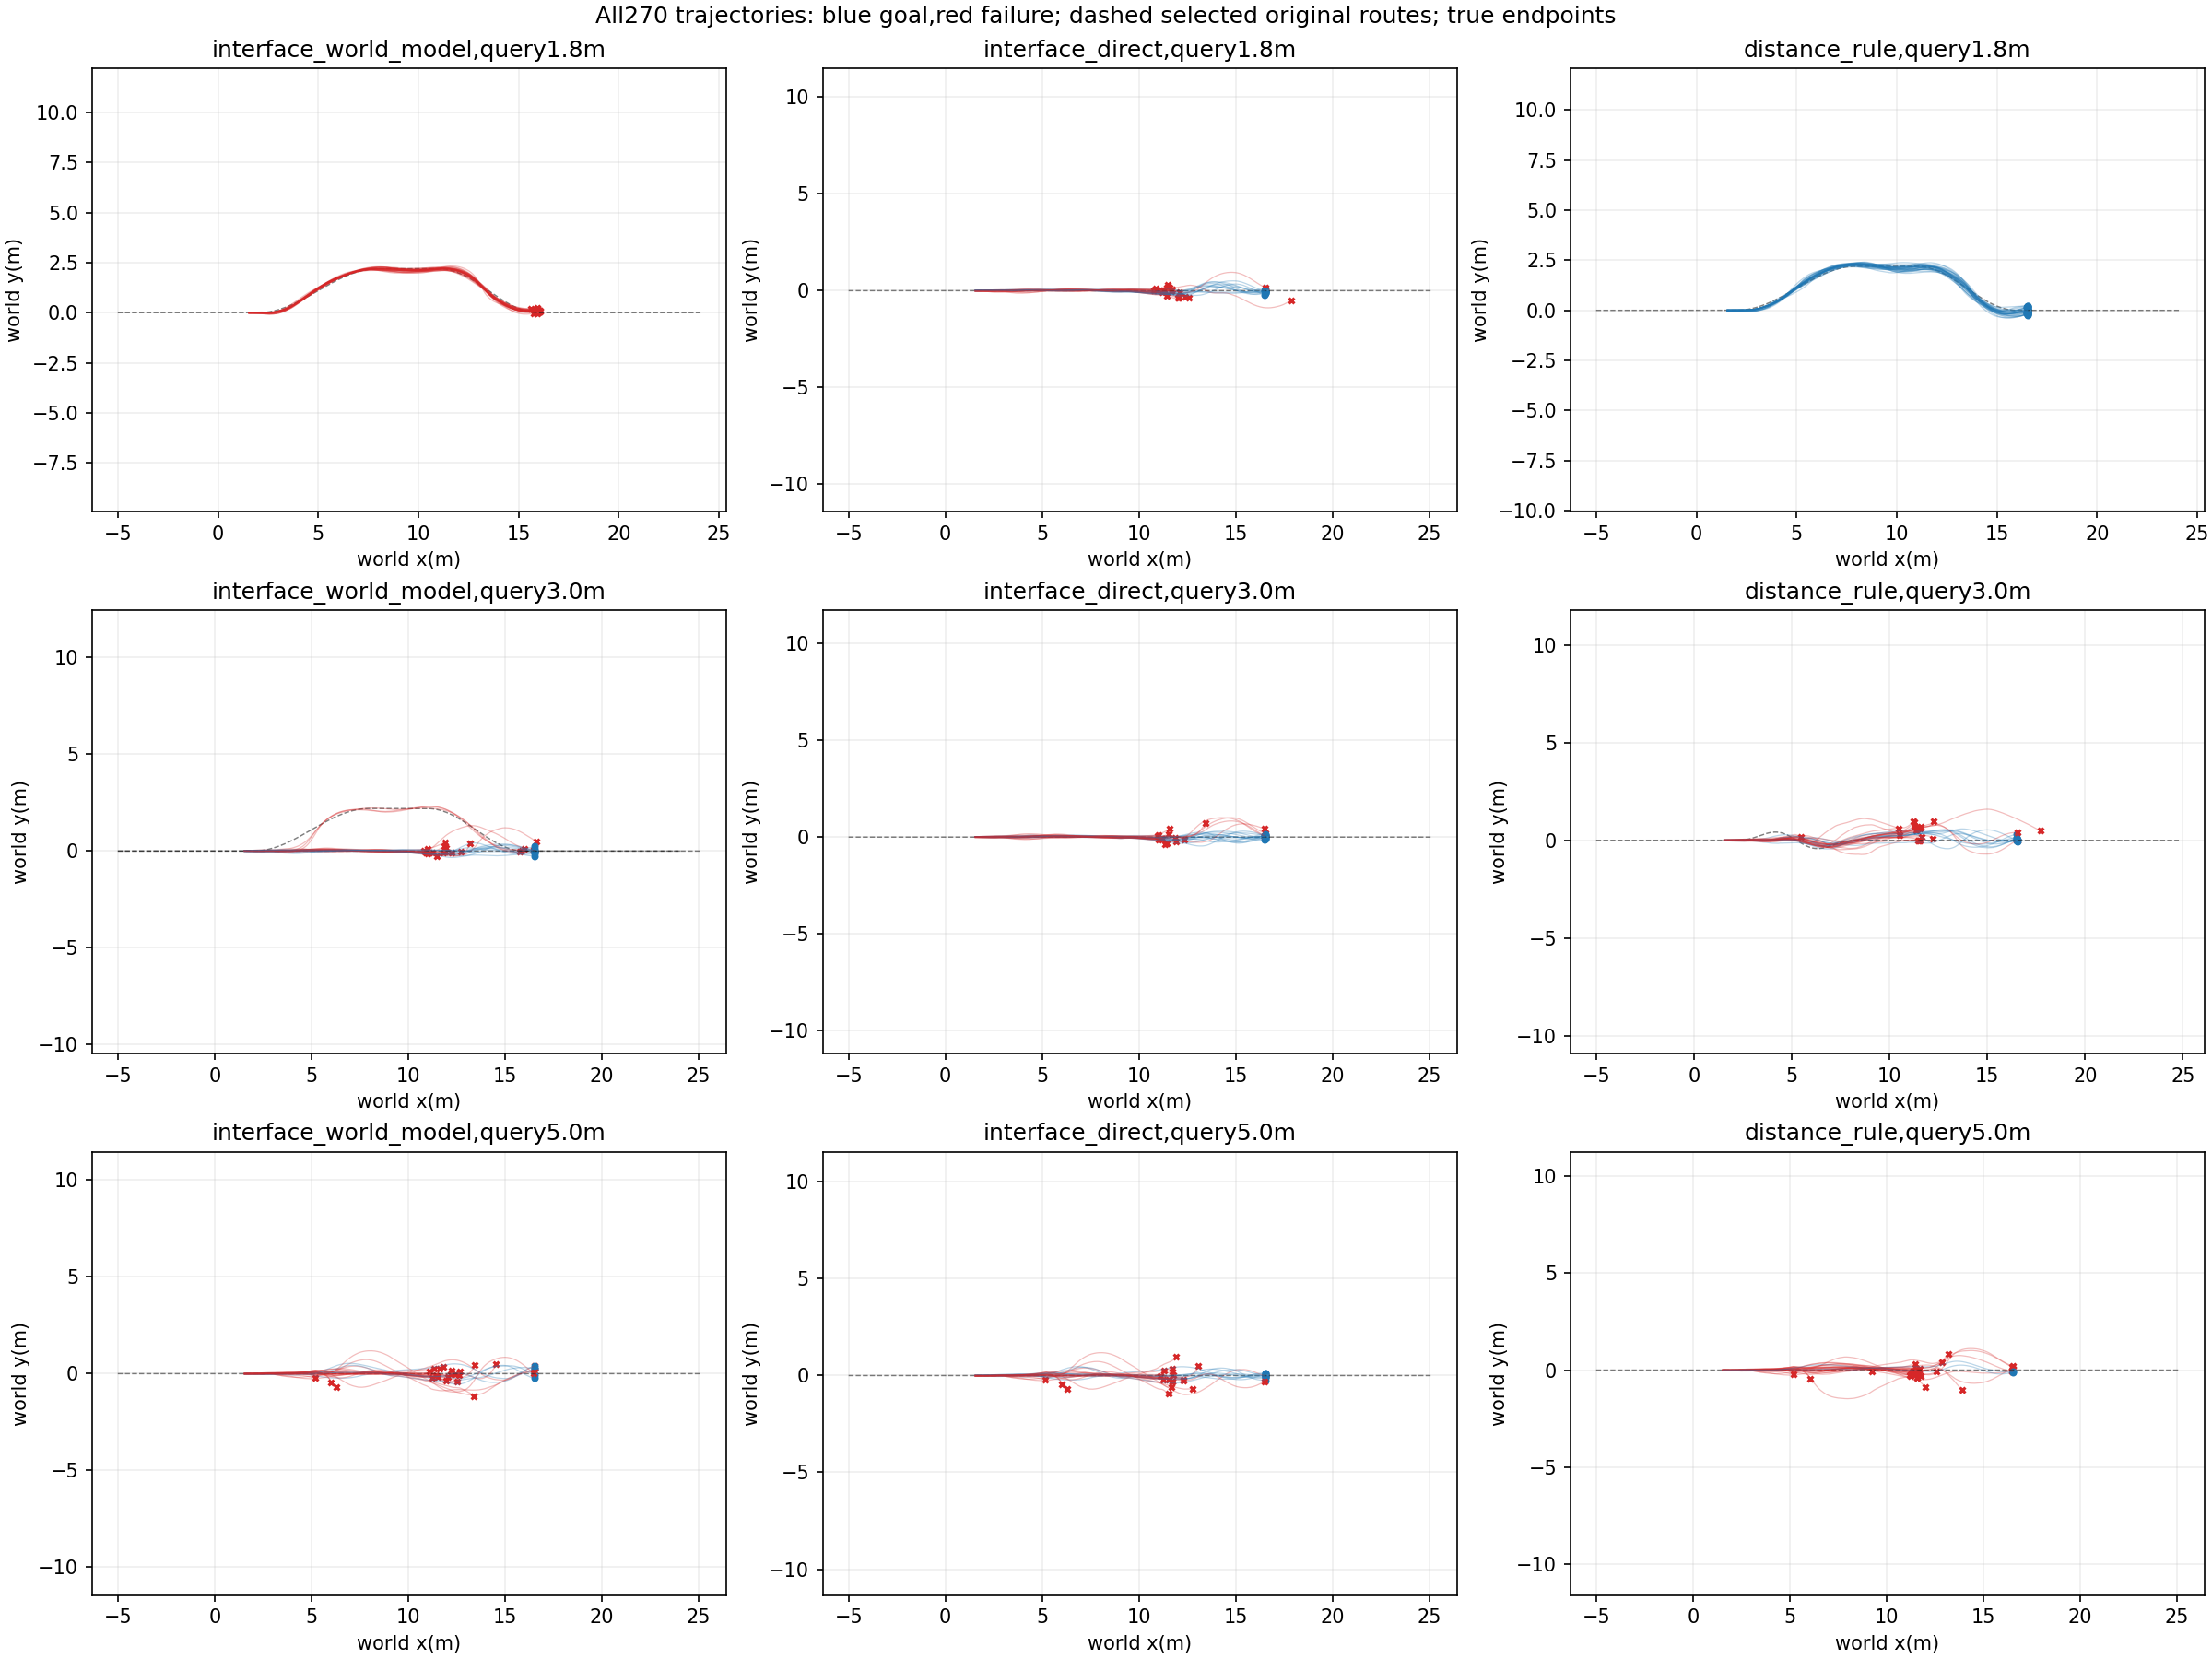
\includegraphics[width=.96\textwidth]{xy_all.png}
\caption{All 270 actual XY executions and selected reference routes, grouped by query position and method. Successful and failed trajectories are retained and terminate at their recorded endpoints. Each method has 30 episodes per position from ten independent conditions with three slot-crossed repetitions.}
\label{fig:xy}
\end{figure*}
\begin{table}[t]
\centering\small
\caption{Actual complete tasks. Each cell at a query position contains ten independent roots with three repetitions.}
\begin{tabular}{lrrr}\toprule
Query $x$ (m)&Interface&Direct&Distance\\\midrule
1.8&0/30&11/30&30/30\\
3.0&10/30&13/30&9/30\\
5.0&5/30&9/30&2/30\\\midrule
Total&15/90&33/90&41/90\\
Road violations&9/90&13/90&22/90\\
Mean query (ms)&6.402&3.506&2.653\\\bottomrule
\end{tabular}
\label{tab:online}
\end{table}
Table~\ref{tab:online} shows a clear overall deficit. The interface model gains 13 and loses 39 matched episodes relative to the rule. Its mean condition-level completion difference is $-0.289$, with a root-bootstrap 95\% interval of $[-0.400,-0.178]$. Against direct success, it gains five and loses 23; the difference is $-0.200$, with interval $[-0.344,-0.067]$. All 90 paired query root states are exactly equal in each comparison. The deficit therefore cannot be dismissed as a mismatch in the recorded query states.

The interface completes 5/30, 3/30, and 7/30 across the three slot rotations; the rule completes 13/30, 14/30, and 14/30. The full panel uses 1,080,000 physical environment steps and 268.06~s summed simulation wall time. Mean query times are below one control period, but a 20-ms physical publication delay is still propagated. This measured result does not establish an architecture-independent latency bound.

\subsection{Why prediction quality did not yield useful ranking}
The interface selects 33 detours, all at 1.5~m/s and $\alpha=0$, and all time out. The other 57 selections are straight crossings. In TRAIN alone, this detour candidate has zero goals in 20 executions yet a mean predicted completion probability of 0.238. A 1.8~m/s, $\alpha=0$ detour has 16/20 goals and mean predicted probability 0.287. The ground head therefore poorly separates useful actions even before online evaluation.

An independently fitted ground head with the same hidden widths and 250-epoch budget improves ground DEV Brier from 0.16439 to 0.15916, but worsens historical transfer from 0.20611 to 0.20728. The zero-success candidate remains overestimated (TRAIN mean 0.34432). A development retest on the same 30 roots completes 14/90, against 30/90 direct and 42/90 rule; all 29 chosen detours time out. Only four interface choices change. The unchanged comparators also vary across batches, precluding a causal interpretation of the 15-to-14 change alone. Average calibration and fewer road violations do not compensate for selecting actions that time out.

\subsection{Changing the task after handoff}


A separate retrospective diagnostic reruns eight historical branches from four original roots in the same environment slots. At measured handoff, the controller receives either the straight reference or a left/right $0.6$-m lateral excursion over $x=12$--$16$~m returning to the same goal. The reference switch does not restore physical state. Terrain, corridor half-width, goal, cold initialization, and posthandoff speed/preference remain fixed. The three variants complete 2/8, 2/8, and 1/8 tasks, respectively, with six handoffs each.

Four sources have identical recorded incoming roots, observations, controller histories, actions, contact modes, and handoff times across variants, without prior road violation. Their outcomes differ (Table~\ref{tab:tasks}). Two other handoff sources have unequal incoming physical records and are excluded only from same-state interpretation, not from aggregate task counts; two never hand off. Equality of recorded quantities does not assert hidden solver-state equivalence.
\begin{table}[t]
\centering\footnotesize
\caption{Four matched historical handoff sources. G: goal; T: timeout; R: road violation; P: physical/domain termination.}
\begin{tabular}{lrrrr}\toprule
Source&Straight&Left&Right&Fixed-context score\\\midrule
1&G&T&G&.16370\\
3&G&G&T&.40342\\
5&P&P&P&.09409\\
7&R&G&T&.37005\\\bottomrule
\end{tabular}
\label{tab:tasks}
\end{table}
Source 7 is a positive continuation example: the left reference completes the task from a recorded incoming state that fails the straight corridor. Conversely, source 1 loses completion under the left task. These differences include deadline and corridor requirements, not only balance. The frozen downstream predictor produces the same score for each source across tasks because downstream geometry is absent from its input. This diagnostic supports task-dependent handoff compatibility and identifies a missing conditioning variable; it does not validate the predictor on changed tasks or establish an adaptive-planning benefit.

\subsection{Task-conditioned continuation extension}
We subsequently collected 540 full-prefix executions: the original 12 roots, 15 straight-crossing approach candidates, and three downstream routes. Straight, left, and right tasks complete 36, 17, and 18 of 180 episodes, respectively. Each yields 122 handoffs without prior road violation. The original eight TRAIN and four DEV roots give 234 TRAIN and 132 DEV conditional outcomes, keeping all task variants of a root together.

The extended downstream input appends 19 known-road features to the 39-dimensional handoff descriptor. Six forward world-$x$ offsets (0, 0.5, 1, 2, 3, and 4~m) provide lateral displacement, heading error, and curvature; the final feature is corridor half-width. No task identifier is supplied. The interface assumes downstream paths monotone in world $x$; width remains fixed in these experiments. Three 64--32 networks are fitted for 200 epochs with the same grouped selection as a state-only ablation on the new data.

The task-conditioned model has DEV Brier 0.10827 versus 0.10290 for the state-only fit and 0.14072 for a constant prior. Straight/left predictions improve slightly, but right-task error increases. On the four previously inspected matched sources in Table~\ref{tab:tasks}, predicted probabilities vary across tasks but straight is ranked first in every case. Source 7 receives 0.107, 0.076, and 0.044 for straight, left, and right, missing its observed left-only success. Thus the geometric input is functional, but improved prediction or task selection has not been established. Online selection is evaluated separately below.

\subsection{Measured-state selection and joint feedback}
An isolated downstream panel assigns 15 straight-approach commands across 30 new roots, with three crossed-slot repetitions per method. Task-conditioned selection completes 13/90, state-only 15/90, and fixed straight 14/90. Among 60 task-conditioned handoffs, straight/left/right are selected 34/19/7 times and complete 12/1/0 tasks. All 180 route publications match their declared 20-ms delay and logged route. Only 6/60 feedback/fixed incoming descriptors match exactly, preventing causal attribution of the one gained and two lost episodes. This panel tests downstream selection with preassigned approach, not joint optimization.

The final panel evaluates Eq.~\eqref{eq:joint} on a separately frozen set of 30 roots drawn from the same ranges, with three crossed-slot repetitions. At $x=3$~m, joint-open selects among 15 straight-crossing approach commands and three downstream roads. Joint-feedback performs the same query and revises the downstream road at measured handoff. The fixed comparator uses 2.0~m/s, $\alpha=0.5$, and straight continuation. All controllers, physical conditions, goal criteria, and the ten-second horizon are unchanged. Models are frozen; this panel is not compared numerically as a matched improvement over the earlier cohorts.

\begin{figure*}[t]
\centering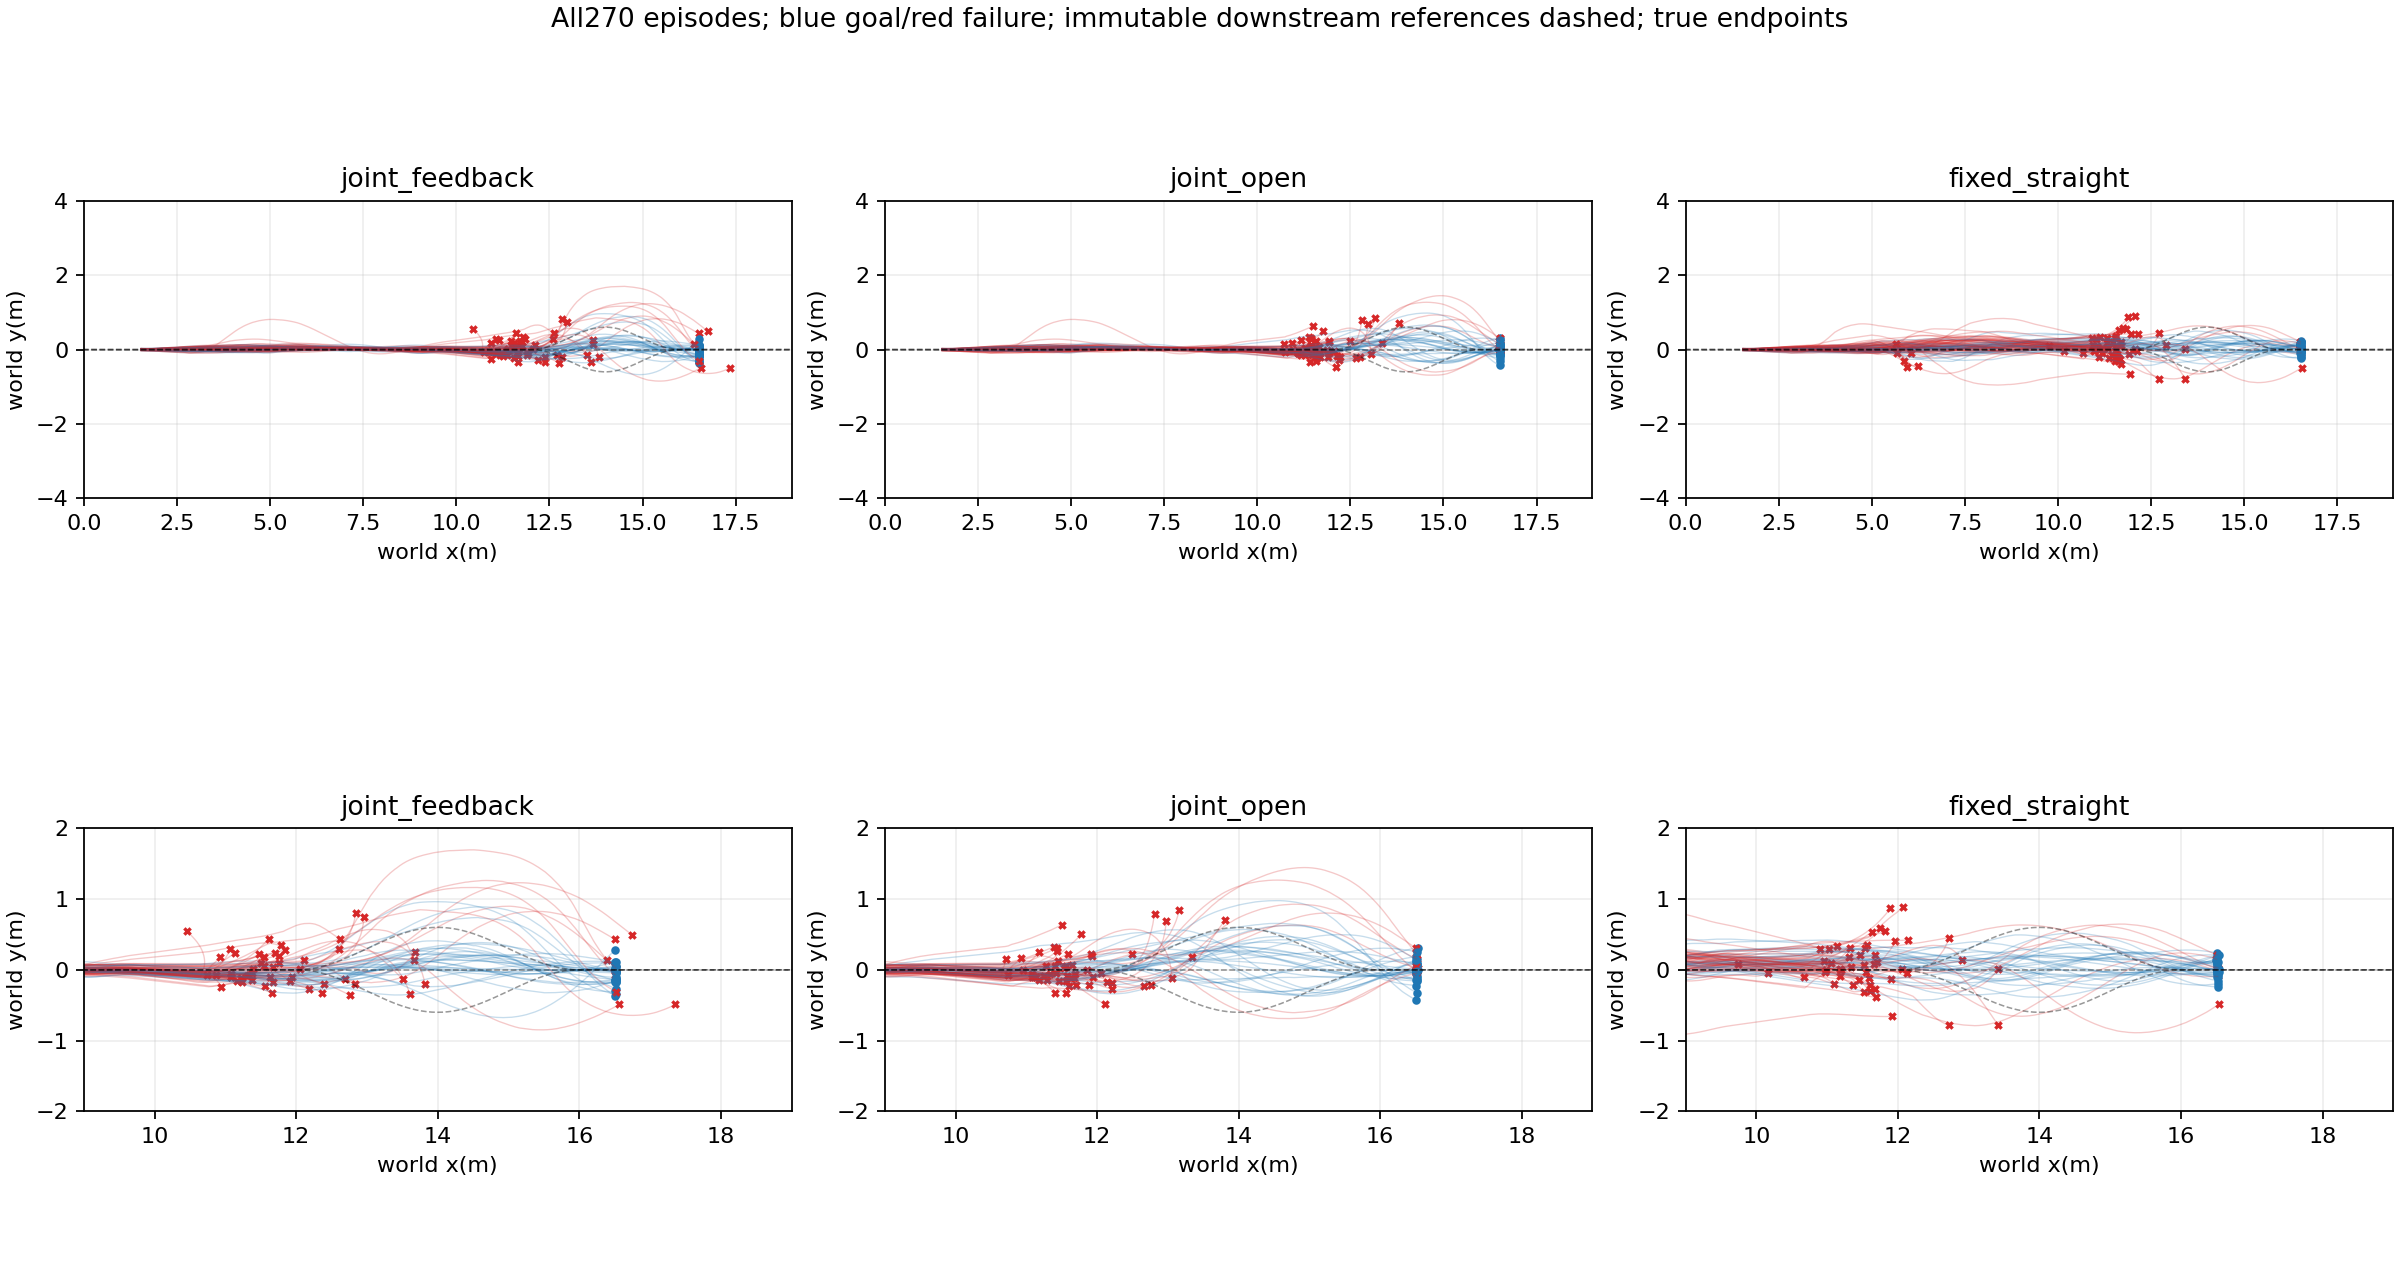
\includegraphics[width=.96\textwidth]{../evidence/chapter3_joint_handoff_online/xy_all.png}
\caption{All 270 joint-panel actual XY trajectories, with downstream references dashed. Top: full task; bottom: handoff vicinity. Blue denotes goal completion and red failure; trajectories end at their true endpoints. All upstream failures remain in the task denominator.}
\label{fig:joint}
\end{figure*}
\begin{table}[t]
\centering\small
\caption{Frozen joint-panel execution: 30 roots and three repetitions per method. Road violations include earlier approach violations.}
\begin{tabular}{lrrr}\toprule
&Feedback&Open plan&Fixed\\\midrule
Goal&30/90&28/90&28/90\\
Valid handoffs&88/90&88/90&77/90\\
Road violations&10/90&9/90&14/90\\
Handoff revisions&44&0&0\\
Goals after revision&11&0&0\\\bottomrule
\end{tabular}
\label{tab:joint}
\end{table}
Both joint methods choose 1.5~m/s and $\alpha=0$ in all 90 episodes. Their advance downstream plans are 72 straight and 18 left. Thus the offered approach grid does not imply demonstrated state-dependent speed/preference selection. Feedback changes 44 plans at actual handoff; eleven revised executions reach the goal. Of the final 52/35/2 straight/left/right choices, 26/3/1 complete. Figure~\ref{fig:joint} and Table~\ref{tab:joint} demonstrate physical execution, including non-straight continuations, rather than counterfactual rescue.

Feedback gains 16 and loses 14 episodes against either comparator. The mean root-level difference is 0.0222; 5,000 root-bootstrap samples give 95\% intervals of $[-0.1111,0.1556]$ against open plan and $[-0.0889,0.1333]$ against fixed. Only 1/89 paired handoff descriptors match exactly against open plan and 0/80 against fixed. Accordingly, neither superiority, equivalence, nor causal rescue is established. Mean upstream queries take 7.899/7.775/0.670~ms and handoff queries 0.434/0.255/0.261~ms for feedback/open/fixed, respectively. All 259 handoff publications match the recorded route and 20-ms delay. Recorded-input replay reproduces all 180 joint score vectors and planned routes exactly. The panel uses 1,066,320 physical environment steps and 275.77~s summed simulation wall time, without fitting or policy training. Per-lane timing is not a serial-batch real-time guarantee; online delay also differs from immediate-switch downstream training.

\section{Discussion}
The two-interface formulation exposes what the planner predicts: whether a lawful handoff will occur, the state and time delivered at that handoff, and the conditional outcome under a specified downstream controller. It removes the need to treat a nearly deterministic controller-switch event as a learned intermediate hazard. It also avoids multiplying marginal contact and goal probabilities whose failure events overlap. These structural choices improve the definition of the estimator, but the online results show that they do not establish a planning advantage.

Several boundaries remain. The initial conditional model uses fixed cold initialization and a straight downstream road; the extension includes three road geometries at one width. It does not measure a recoverability margin or distinguish states that can be rescued by a short correction. A nominal ground-motion envelope was examined separately, but many successful two-second continuations did not enter it; envelope membership is therefore not adopted as a necessary capture condition. Measured initialization also failed to improve an eight-source same-slot diagnostic, which does not rule out useful initialization from genuine controller histories.

The relationship to skill repair remains a hypothesis requiring matched interface evidence. Earlier whole-task substitution yielded 34/240 completions with the original jump skill and 35/240 with RB400. This denominator correctly measures system-level utility, including failures before the skill is activated. Conditional skill comparisons at matched legal entrances answer a different question and should supplement, rather than replace, the whole-task result.

The immediate methodological gap is candidate ranking, especially the ground branch. The independent ground-head fit and development retest leave the dominant failure unresolved without changing task deadlines or retraining the jump skill. If the present 30 roots inform that correction, they become development evidence for the repaired model. The route intervention and measured-state selection demonstrate task dependence and executable feedback. Joint selection and measured-state revision now execute physically, but the small completion difference is uncertain and speed/preference choices collapse to one setting. The fixed-width, three-road extension does not validate new-map or unseen-width transfer. No hardware or new-map generalization is established.

\section{Conclusion}
We implemented a handoff-conditioned world model for composing frozen driving and jumping controllers on a known off-road map. The model predicts a physical handoff distribution and evaluates its downstream consequences, with explicit training targets and a finite-candidate execution interface. The new online panel confirms completed jump--ground tasks but shows lower completion than both a direct classifier and a distance rule. A poorly discriminating ground-route head accounts for a substantial observed failure mode. A task-conditioned extension additionally chooses downstream roads at measured handoff, including a successful non-straight continuation, without establishing improved aggregate completion. Joint approach--road selection with measured-state revision completes 30/90 tasks against 28/90 for both open-plan and fixed controls, without establishing superiority. The study separates executable feedback from improved selection; recoverability margins and reliable state-dependent approach selection remain open.

\begin{thebibliography}{99}
\bibitem{burridge1999}R. R. Burridge, A. A. Rizzi, and D. E. Koditschek, ``Sequential composition of dynamically dexterous robot behaviors,'' \emph{Int. J. Robotics Research}, vol. 18, no. 6, 1999, doi:10.1177/02783649922066385.
\bibitem{xin2020}S. Xin and S. Vijayakumar, ``Online dynamic motion planning and control for wheeled biped robots,'' arXiv:2003.03678, 2020.
\bibitem{lee2024}J. Lee, M. Bjelonic, A. Reske, L. Wellhausen, T. Miki, and M. Hutter, ``Learning robust autonomous navigation and locomotion for wheeled-legged robots,'' \emph{Science Robotics}, vol. 9, no. 89, 2024, doi:10.1126/scirobotics.adi9641.
\bibitem{chua2018}K. Chua, R. Calandra, R. McAllister, and S. Levine, ``Deep reinforcement learning in a handful of trials using probabilistic dynamics models,'' in \emph{NeurIPS}, 2018.
\bibitem{yang2020}Y. Yang, K. Caluwaerts, A. Iscen, T. Zhang, J. Tan, and V. Sindhwani, ``Data efficient reinforcement learning for legged robots,'' in \emph{Proc. Conference on Robot Learning}, PMLR 100, 2020, pp. 1--10.
\bibitem{wu2022}P. Wu, A. Escontrela, D. Hafner, K. Goldberg, and P. Abbeel, ``DayDreamer: World models for physical robot learning,'' arXiv:2206.14176, 2022.
\end{thebibliography}
\end{document}
